\section{Accuracy of the model}
It is certainly important to investigate the accuracy of our model. 
However, performing an error analysis on a system with 1000 particles that strongly interact with each other is cumbersome. 
Therefore, we have only investigated our model on a two bodies system, which consists of a planet of 1 $M_{\oplus}$ rotating around the sun.\\
\\
The choice of a two bodies system has other desired properties as well, namely there is no collision, which means that the only energy contribution in the system is the kinetic energy and the potential energy, which makes energy calculation much simpler. Also, with just two bodies, there is no barnes-hut involved. In this way, Leapfrog is the only major factor concerning the accuracy of this system and we hope to get an idea about the accuracy of our general model by investigating LeapFrog in this special case.

\subsection{Elliptical orbit and conservation of energy}
One way to investigate the accuracy of the model is to check whether the calculations make sense physically. Due to Kepler's law, we expect the orbit of our planet around the sun should be elliptical. 
Also, since we are dealing with an isolated system, the total energy of the system, must be conserved. 
Therefore, it is meaningful to investigate whether our model satisfies these two properties.\\ 
\\
The total energy of the system is \cite{Energy}
\[E_{tot}=\frac{1}{2}mv_{planet}^2+\frac{1}{2}Mv_{sun}^2-\frac{GmM}{r}\]
With $m$ and $M$ the mass of the planet and the sun, $r$ the distance between the planeet and the sun.\\
\\
By considering the motion of the relative position, we can transform this two-bodies problem into a single body problem\cite{reducedmass}. To do this, we first choose the center of mass to be the origin, which was also one of the assumption in our model, this gives:
\begin{align}
m_1\vec{r_1}+m_2\vec{r_2}=\vec{0}\label{eq:CM} 
\end{align}
with $m_i$, $\vec{r_i}$ the mass and position of $i$-th particle. We then set
\begin{align*}
\vec{r}&=\vec{r_1}-\vec{r_2}\\ 
	   &=\vec{r_1}+\frac{m_1}{m_2}\vec{r_1}\\
	   &=\vec{r_1}(1+\frac{m_1}{m_2}) 
\end{align*}
In which we used \ref{eq:CM} for the substitution. If we now consider the motion of particle 1:
\begin{align*}
m_1\frac{d^2\vec{r_1}}{dt^2}=\vec{F_1}
\end{align*}
Then by subsitution, we obtain:
\begin{align*}
\frac{m_1\cdot m_2}{m_1+m_2}\cdot\frac{d^2 \vec{r}}{dt^2}&=\vec{F_1}\\
\mu\frac{d^2 \vec{r}}{dt^2}&=\vec{F_1}
\end{align*}
The quantity $\mu=\frac{m_1m_2}{m_1+m_2}$ is known as the reduced mass. We have now transformed a two bodies problem into an one body problem, in which $\mu$ can be viewed as the mass of this new body. This one body system is equivalent to the original two bodies system, since knowing $\vec{r}$ would give us $r_1$ and $r_2$. \\
\\
By substituting $\mu$ into the total energy equation, we can also obtain an equivalent energy equation for the one body problem:
\begin{align}
E_{tot}=\frac{1}{2}\mu |\vec{v}|^2-\frac{GM_{tot}}{|\vec{r}|}
\end{align}
With $M_{tot}=m_1+m_2$. It is not surprising that the equivalent energy formula looks like the energy formula for one particle with mass $\mu$. Now that we have derived our formula. We will perform the simulation with a planet of mass $m=1M_{\oplus}$, and the sun has mass $M=3.33\cdot 10^5 M_{\oplus}$. Since $M\gg m$, and $m=1$ in earth mass unit(we will calculate energy/earth mass), we have that $M_{tot}\approx M$ and $\mu\approx 1$. Also $|\vec{r}|\approx |\vec{r}_{planet}|$.\\
\\
After performing the simulation, it turns out that if the planet has a distance of more than $1$AU to the center of mass, that the energy is very well conserved and smooth, circular orbit is obtained(see Appendix). The most interesting case is when the distance is less than $1$ AU, because then we observed some inaccuracy in the numerical solution of the orbit. This is shown in Figure \ref{fig:Planet1AUdt1} 
\begin{figure}[H]
\centering
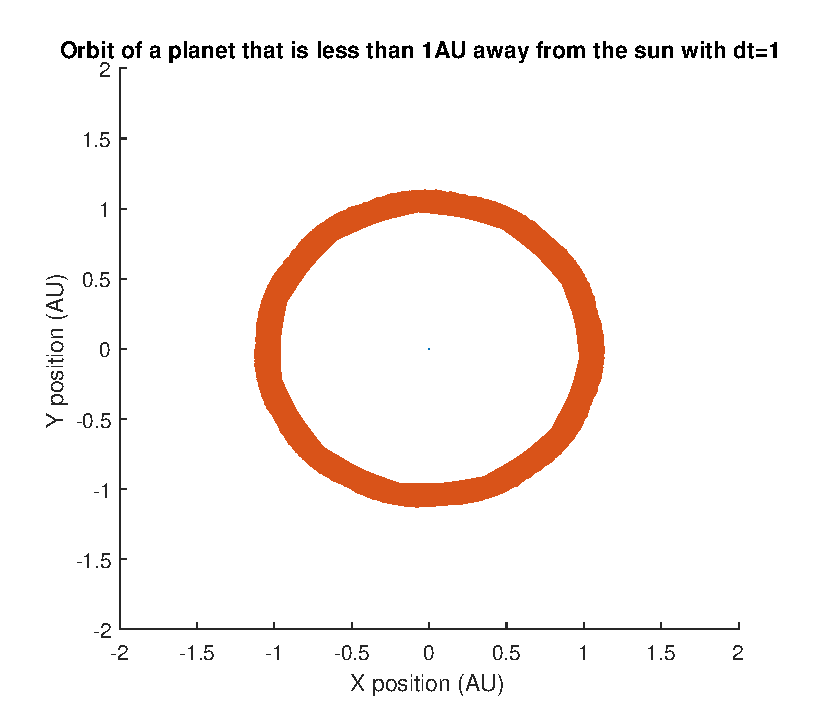
\includegraphics[width=0.6\textwidth]{Planeet_1AU_dt1_100jaar.eps}
\caption{Orbit of a planet of 1 $M_{\oplus}$ with a distance less than 1AU from the sun, integrated with $dt=1$ month over $100$ years.}
    \label{fig:Planet1AUdt1}
\end{figure}
\leavevmode
\\
Also, a calculation of energy shows that the energy is not exactly conserved:
\begin{table}[htb]
\centering
\caption{The total energy of the system, which consists of a planet rotating less than 1AU away from the sun. The energy is calculated after each 100 time steps.}
\label{my-label}
\begin{tabular}{|l|l|l|l|l|l|l|l|}
\hline
k-th timestep &0 &100 & 200 & 300 & 400 & 500 & 600\\ \hline
$E_{tot}$     & -0.1360 & -0.0983 & -0.0966 & -0.0967 & -0.0980 & -0.1008 & -0.1041\\ \hline
k-th timestep & 700 & 800 & 900 & 1000 & 1100  & 1200& \:\:\:\:\:\:\textbackslash   \\ \hline
$E_{tot}$& -0.1066 & -0.1095 & -0.1111 & -0.1122 & -0.1134 & -0.1127&\:\:\:\:\:\:\textbackslash  \\ \hline
\end{tabular}
\label{tab:Planet1AUEnergy}
\end{table}

It is not surprising that the simulation becomes inaccurate if the planet is close enough to the origin.
Because these planets have a much shorter orbital period than the earth. It is known that the stability of Leapfrog, when applied to an oscillatory system, is $\Delta t\leq 2/\omega$, with $\omega$ the angular frequency \cite{StabLeapfrog}. This means that for planets that have a shorter orbital period and thus larger $\omega$, the stability of Leapfrog is lost if $\Delta t$ is not small enough.\\

Another remarkeble thing we observed in Figure \ref{fig:Planet1AUdt1} is, that the plot of all orbits within 100 years together form a circle with a very thick boundary. This can mean two things: Either the orbit is bounded, or the orbit is slowly collapsing to (or expanding away from) the origin. Since our energy calculation shows that energy is still quite conserved, we conclude that the orbit is bounded. This shows that even though LeapFrog is unstable when $\Delta t=1$ is used for a planet with a distance around(or less than) 1 AU, the instability is not too ``bad", which means that the round-off error is bounded. The remarkeble property that LeapFrog is weakly unstable if $\Delta t$ is not too large is also reported in several other literatures(\cite{Energy} and \cite{Leapfrogsympletic}).\\
\\ 
As expected, if we chose to integrate with $dt=0.5$ or $dt=0.25$, the accuracy of the orbit is greatly improved:

\begin{figure}[H]
	\centering
	\begin{subfigure}{0.45\textwidth}
	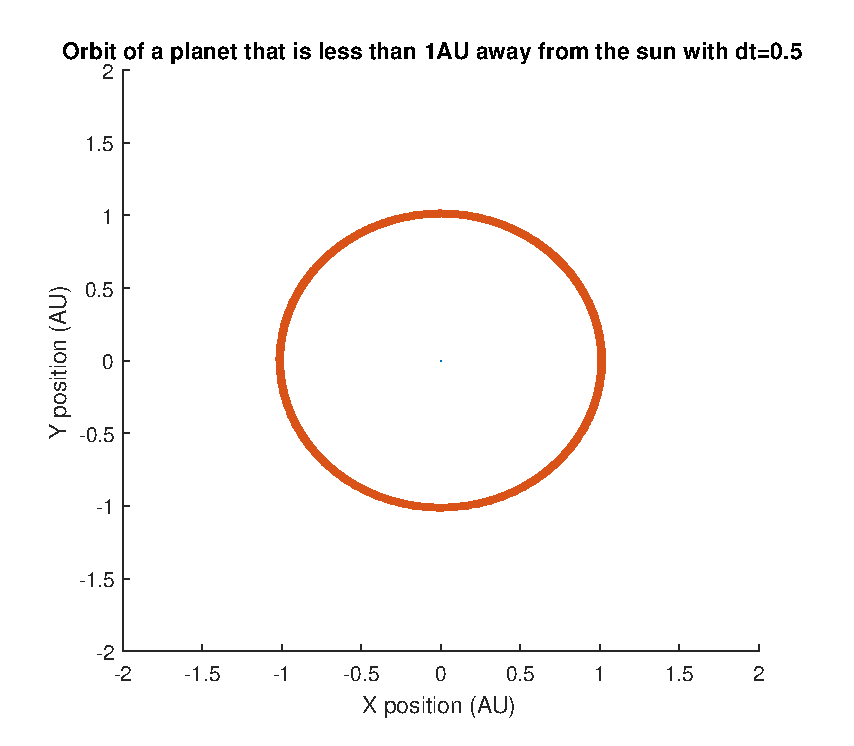
\includegraphics[width=\textwidth]{Planeet_1AU_dt05_100jaar.eps}
	\caption{Orbit calculation with $dt=0.5$}
	\end{subfigure}
	~
	\begin{subfigure}{0.45\textwidth}
	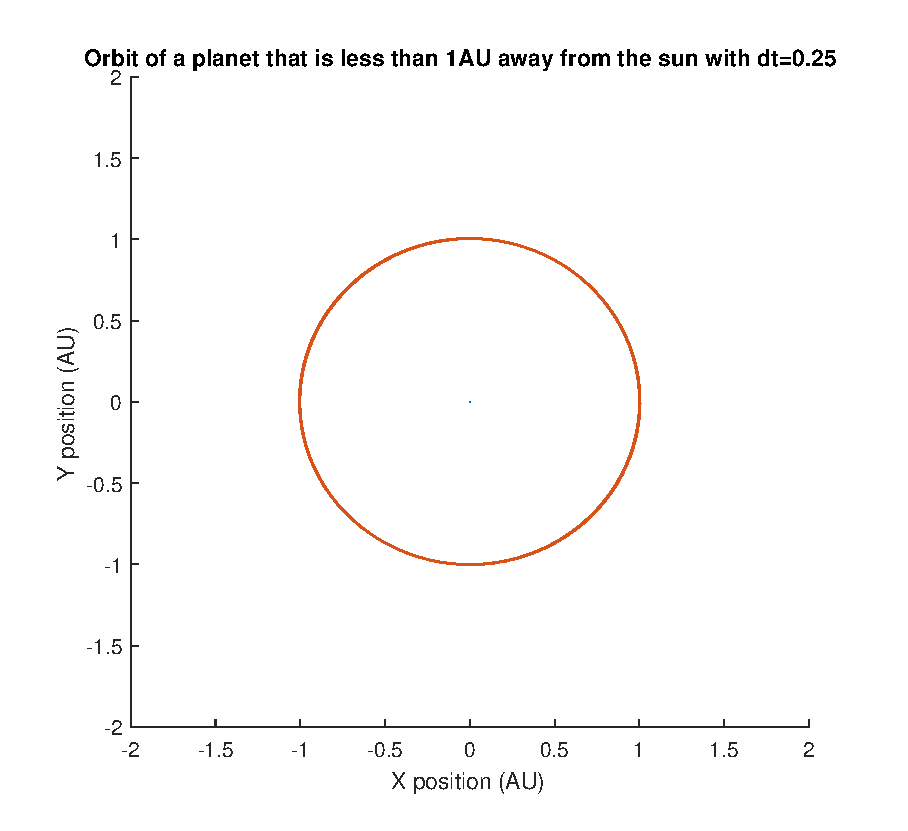
\includegraphics[width=\textwidth]{Planeet_1AU_dt025_100jaar.eps}
	\caption{Orbit calculation with $dt=0.25$}
	\end{subfigure}
	\caption{Orbit of a planet of 1 $M_{\oplus}$ with a distance less than 1 AU from the sun, integrated with $dt=0.5$ month and $dt=0.25$ month over $100$ years.}
\end{figure} 
\leavevmode
\\
Although the orbits of the planets in our general simulations are circular, it is also interesting to investigate whether LeapFrog conserves energy for a planet that has an elliptical but not circular orbit. This is interesting because the distance $r$ to the center of mass is now time-dependent. The results are as follow:
\begin{figure}[H]
\centering
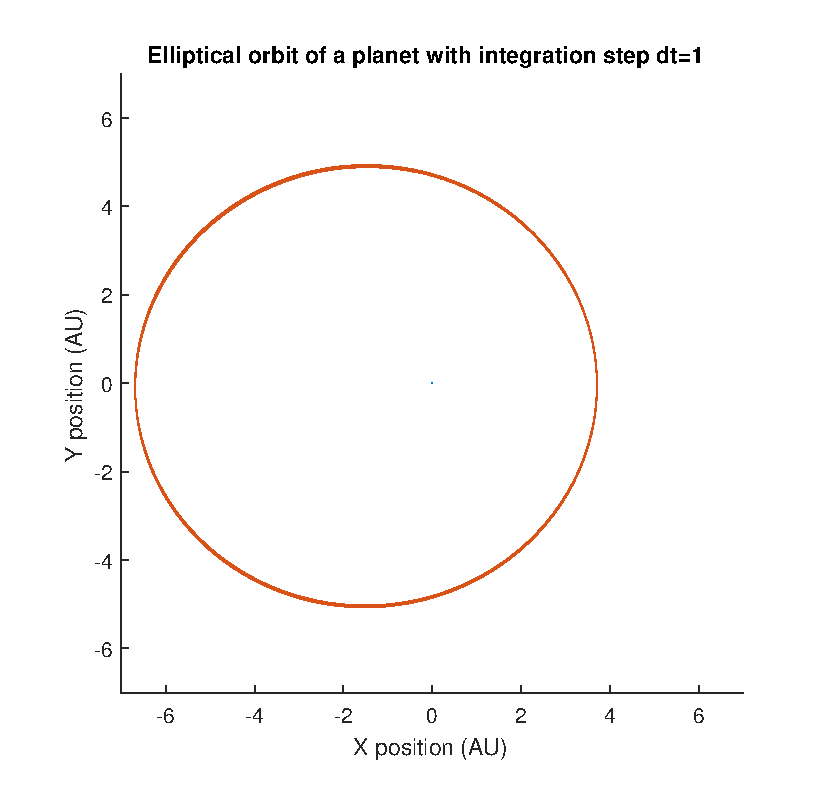
\includegraphics[width=0.8\textwidth]{elliptisch100jaar.eps}
\caption{Elliptical orbit of a planet of 1 $M_{\oplus}$, integrated with $dt=1$ month over $100$ years. The sun lies practically at (0,0), together with the center of mass}
    \label{fig:Planetellipse}
\end{figure}
\begin{table}[htb]
\centering
\caption{The total energy of the system, which consists of a planet following an elliptical orbit about the sun. The energy is calculated after each 100 time steps.}
\label{my-label}
\begin{tabular}{|l|l|l|l|l|l|l|l|}
\hline
k-th timestep &0 &100 & 200 & 300 & 400 & 500 & 600\\ \hline
$E_{tot}$     &  -0.0262&   -0.0261&   -0.0262&   -0.0261&   -0.0260&   -0.0261&   -0.0261 \\ \hline
k-th timestep & 700 & 800 & 900 & 1000 & 1100  & 1200& \:\:\:\:\:\:\textbackslash   \\ \hline
$E_{tot}$& -0.0260  & -0.0261  & -0.0261  & -0.0261  & -0.0261& -0.0262&\:\:\:\:\:\:\textbackslash  \\ \hline
\end{tabular}
\label{tab:PlanetellipseEnergy}
\end{table}
As we can see in Figure \ref{fig:Planetellipse}, the orbit, although still quite circular, is not a circle around the star(which lies practically at $(0,0)$). This means that the distance to the star is indeed time-dependent. We see from table \ref{tab:PlanetellipseEnergy} that the energy is still very well conserved with LeapFrog. During this simulation, we have observed that for the stability of LeapFrog, smaller $\Delta t$ is required than the usual case with circular orbit around $(0,0)$. We think this is because that at certain time-interval $[t_j,t_{j+1}]$, the distance of the planet is less than $1$ AU during this interval. 
\subsection{Richardson Extrapolation}
Another more mathematical way to investigate the error of our integration is with Richardson Extrapolation. 
Let $Q(h)$ be the approximation using step size $h$. 
Then, the Richardson Extrapolation formula \cite{Richardson} gives an estimate for the order $p$ of the used numerical method:
\[\frac{Q(2h)-Q(4h)}{Q(h)-Q(2h)}=2^p\]

Therefore, we calculated the final position(thus after 10 years) of a planet which starts in a distance around 5AU from the sun, with $dt=1$, $dt=0.5$ and $dt=0.25$ and applied the Richardson Extrapolation formula. 
The result is shown in Table \ref{tab:Richardson5AU}:

\begin{table}[htb]
\centering
\caption{The final position of a planet that is around 5AU away from the sun, calculated with three different step size, namely $dt=1$, $dt=0.5$ and $dt=0.25$.}
\begin{tabular}{|l|l|l|l|}
\hline
dt (month)&1&0.5&0.25\\ \hline
x position (AU)&-3.2505&   -3.1469&   -3.0978\\ \hline
y position (AU)&   -3.8003&   -3.8859&   -3.9250\\ \hline
\end{tabular}
\label{tab:Richardson5AU}
\end{table}
\leavevmode
\\
For the order of the x position, denoted as $p_x$, the formula gives $p_x\approx 1.0782$.\\
For the order of the y position, denoted as $p_y$, the formula gives $p_y\approx 1.1304$.\\ 

This is very surprising result, because Leapfrog is known as a second order method. We do not know the reason yet.
\subsection{Comments about accuracy of our results}
What does this analysis of two bodies says anything about our results with for example 1000 bodies? From the above observation, we saw that the integration is inaccurate for planets too close to the sun. Therefore, in our simulations with more bodies, we avoid this inaccuracy by conditioning the initial distance of each planets to the center of mass to be more than 1 AU, since we are integrating with $dt=1$. Of course, this comes with the price that our model is less realistic. Certainly, we could have chose a smaller $dt$ for planets close to the origin, but that would also require somewhat more programming work.\\

The circular orbit that we observed with only one planet implies that we are integrating correctly(there is still a error of order 1, but at least we obtained a reasonable solution). With more bodies, we will also have collisions, in which we used Euler Forwards to determine the condition for collisions. So we expect that in our results, the order of the error for the position of the bodies would still be 1.\\

It would not be wise to try to calculate the total energy of a solar system for large $N$. First of all, although the total energy in the system is conserved, due to collisions between planets, the total energy would have other contribution factors than just kinetic energy and gravity potential energy, which makes it difficult to calculate. The second difficulty lies in the fact that the energy calculation, is just like the force, has complexity $\mathcal{O}(N^2)$, which requires huge amount of calculation for large $N$.